% Options for packages loaded elsewhere
\PassOptionsToPackage{unicode}{hyperref}
\PassOptionsToPackage{hyphens}{url}
%
\documentclass[
  ignorenonframetext,
]{beamer}
\usepackage{pgfpages}
\setbeamertemplate{caption}[numbered]
\setbeamertemplate{caption label separator}{: }
\setbeamercolor{caption name}{fg=normal text.fg}
\beamertemplatenavigationsymbolsempty
% Prevent slide breaks in the middle of a paragraph
\widowpenalties 1 10000
\raggedbottom
\setbeamertemplate{part page}{
  \centering
  \begin{beamercolorbox}[sep=16pt,center]{part title}
    \usebeamerfont{part title}\insertpart\par
  \end{beamercolorbox}
}
\setbeamertemplate{section page}{
  \centering
  \begin{beamercolorbox}[sep=12pt,center]{part title}
    \usebeamerfont{section title}\insertsection\par
  \end{beamercolorbox}
}
\setbeamertemplate{subsection page}{
  \centering
  \begin{beamercolorbox}[sep=8pt,center]{part title}
    \usebeamerfont{subsection title}\insertsubsection\par
  \end{beamercolorbox}
}
\AtBeginPart{
  \frame{\partpage}
}
\AtBeginSection{
  \ifbibliography
  \else
    \frame{\sectionpage}
  \fi
}
\AtBeginSubsection{
  \frame{\subsectionpage}
}

\usepackage{amsmath,amssymb}
\usepackage{iftex}
\ifPDFTeX
  \usepackage[T1]{fontenc}
  \usepackage[utf8]{inputenc}
  \usepackage{textcomp} % provide euro and other symbols
\else % if luatex or xetex
  \usepackage{unicode-math}
  \defaultfontfeatures{Scale=MatchLowercase}
  \defaultfontfeatures[\rmfamily]{Ligatures=TeX,Scale=1}
\fi
\usepackage{lmodern}
\ifPDFTeX\else  
    % xetex/luatex font selection
\fi
% Use upquote if available, for straight quotes in verbatim environments
\IfFileExists{upquote.sty}{\usepackage{upquote}}{}
\IfFileExists{microtype.sty}{% use microtype if available
  \usepackage[]{microtype}
  \UseMicrotypeSet[protrusion]{basicmath} % disable protrusion for tt fonts
}{}
\makeatletter
\@ifundefined{KOMAClassName}{% if non-KOMA class
  \IfFileExists{parskip.sty}{%
    \usepackage{parskip}
  }{% else
    \setlength{\parindent}{0pt}
    \setlength{\parskip}{6pt plus 2pt minus 1pt}}
}{% if KOMA class
  \KOMAoptions{parskip=half}}
\makeatother
\usepackage{xcolor}
\newif\ifbibliography
\setlength{\emergencystretch}{3em} % prevent overfull lines
\setcounter{secnumdepth}{-\maxdimen} % remove section numbering


\providecommand{\tightlist}{%
  \setlength{\itemsep}{0pt}\setlength{\parskip}{0pt}}\usepackage{longtable,booktabs,array}
\usepackage{calc} % for calculating minipage widths
\usepackage{caption}
% Make caption package work with longtable
\makeatletter
\def\fnum@table{\tablename~\thetable}
\makeatother
\usepackage{graphicx}
\makeatletter
\def\maxwidth{\ifdim\Gin@nat@width>\linewidth\linewidth\else\Gin@nat@width\fi}
\def\maxheight{\ifdim\Gin@nat@height>\textheight\textheight\else\Gin@nat@height\fi}
\makeatother
% Scale images if necessary, so that they will not overflow the page
% margins by default, and it is still possible to overwrite the defaults
% using explicit options in \includegraphics[width, height, ...]{}
\setkeys{Gin}{width=\maxwidth,height=\maxheight,keepaspectratio}
% Set default figure placement to htbp
\makeatletter
\def\fps@figure{htbp}
\makeatother

\makeatletter
\@ifpackageloaded{caption}{}{\usepackage{caption}}
\AtBeginDocument{%
\ifdefined\contentsname
  \renewcommand*\contentsname{Table of contents}
\else
  \newcommand\contentsname{Table of contents}
\fi
\ifdefined\listfigurename
  \renewcommand*\listfigurename{List of Figures}
\else
  \newcommand\listfigurename{List of Figures}
\fi
\ifdefined\listtablename
  \renewcommand*\listtablename{List of Tables}
\else
  \newcommand\listtablename{List of Tables}
\fi
\ifdefined\figurename
  \renewcommand*\figurename{Figure}
\else
  \newcommand\figurename{Figure}
\fi
\ifdefined\tablename
  \renewcommand*\tablename{Table}
\else
  \newcommand\tablename{Table}
\fi
}
\@ifpackageloaded{float}{}{\usepackage{float}}
\floatstyle{ruled}
\@ifundefined{c@chapter}{\newfloat{codelisting}{h}{lop}}{\newfloat{codelisting}{h}{lop}[chapter]}
\floatname{codelisting}{Listing}
\newcommand*\listoflistings{\listof{codelisting}{List of Listings}}
\makeatother
\makeatletter
\makeatother
\makeatletter
\@ifpackageloaded{caption}{}{\usepackage{caption}}
\@ifpackageloaded{subcaption}{}{\usepackage{subcaption}}
\makeatother

\ifLuaTeX
  \usepackage{selnolig}  % disable illegal ligatures
\fi
\usepackage{bookmark}

\IfFileExists{xurl.sty}{\usepackage{xurl}}{} % add URL line breaks if available
\urlstyle{same} % disable monospaced font for URLs
\hypersetup{
  pdftitle={Accuracy and Prediction},
  pdfauthor={Horacio Gomez-Acevedo},
  hidelinks,
  pdfcreator={LaTeX via pandoc}}


\title{Accuracy and Prediction}
\author{Horacio Gomez-Acevedo}
\date{}

\begin{document}
\frame{\titlepage}


\begin{frame}{Main reference}
\phantomsection\label{main-reference}
Some of the figures and material in this presentation are taken from
(Gareth, James et al., 2015) with permission from the authors: G. James,
D. Witten, T. Hastie and R. Tibshirani
\end{frame}

\begin{frame}{Basic Setup}
\phantomsection\label{basic-setup}
Let's suppose we observe a quatitative response \(Y\) and \(p\)
different predictors \(X_1,\ldots, X_p\), which can be written in the
form \[
Y= f(X) + \varepsilon
\] We assume that the function \(f\) is \textbf{fixed but unknown}, and
\(\varepsilon\) is a \textbf{random error term}, which is independent of
\(X\) and has mean zero (i.e.~its expected value
\(E (\varepsilon) =0\)).

\textbf{Statistical Learning} refers to a set of approaches for
estimating \(f\), for the purpose of either predict future responses or
make inferences about inner relationships within the model predictors.

\begin{block}{Prediction}
\phantomsection\label{prediction}
Let's suppose that a set of input (predictors) is readily available, but
for some financial or practical constrains we cannot estimate the output
\(Y\). We can predict \(Y\) using \[
    \hat{Y} = \hat{f}(X),
\] where \(\hat{f}\) represents an estimate for \(f\) and \(\hat{Y}\)
represent the resulting prediction for \(Y\).

\begin{quote}
Note that this is a very general setting, for instance in (multi)linear
regression, we cannot make predictions outside certain regions.
\end{quote}

\begin{block}{How accurate is \(\hat{Y}\)?}
\phantomsection\label{how-accurate-is-haty}
The accuracy of \(\hat{Y}\) as a prediction for \(Y\) depends on two
quantities + reducible error + irreducible error

The reducible error reflects the leverage that modeler has to pick a
\emph{better} statistical technique for estimation. Even in the case
when we have a perfect estimate of \(f\) (i.e.~\(\hat{Y}=f(X)\)), we
will have \[
|\hat{Y}-Y| = \varepsilon
\] since \(\varepsilon\) does not depend on \(X\). Thus, we cannot
reduce the error introduced by \(\varepsilon\) no matter how well our
estimates are.

Recall that if you have a random variable \(Z\) (with \(E(|Z|)<\infty\)
and \(\mathrm{Var}(Z)<\infty\)), the following relationships hold
\[E(Z^2)= \mathrm{Var}(Z) + (E(Z))^2\] and
\[\mathrm{Var}(aZ+b)= a^2\mathrm{Var}(Z)\]

Now if we consider for a moment that both \(\hat{f}\) and \(X\) are
fixed (\(f\) was already fix but unknown), we have that the average
(expected value) of the squared difference is

\[
\begin{align}
E(Y-\hat{Y})^2&= E(f(X)+ \varepsilon -\hat{f}(X))^2= \mathrm{Var}(f(X)-\hat{f}(X)+ \varepsilon ) + \left(E(f(X)-\hat{f}(X)+\varepsilon) \right)^2 \\
&= \mathrm{Var}(\varepsilon) + \mathrm{Var}(f(X)-\hat{f}(X))+ \left( E(f(X)-\hat{f}(X)) + E(\varepsilon) \right)^2\\
&= \color{red}{\mathrm{Var}(\varepsilon)}+\color{blue}{E\left( f(X)-\hat{f}(X)\right)^2} 
\end{align}
\] The reducible error is colored in blue and the irreducible error is
in red.

Thus, the accuracy will be (lower) bounded by
\(\mathrm{Var}(\varepsilon)\), but this bound is almost never known in
practice.
\end{block}
\end{block}

\begin{block}{Inference}
\phantomsection\label{inference}
In this case we are mainly interested in determined the way that \(Y\)
is affected by changing \(X_1,\ldots,X_p\). This means trying to
understand the relationship between the output and the predictors. For
instance we try to answer questions like

\begin{itemize}
\tightlist
\item
  Which predictors are more important?
\item
  What relationship exist between the response and each of the
  predictors?
\item
  Is the relationship between \(Y\) and predictor \(X_i\) linear, or
  should it be nonlinear?
\end{itemize}
\end{block}
\end{frame}

\begin{frame}{Estimation of \(f\)}
\phantomsection\label{estimation-of-f}
The observations at hand are called \textbf{training data}, because we
will use those observations to find an estimate \(\hat{f}\). Let
\(x_{ij}\) represents the value of the predictor \(j\) for the \(i\)th
observation (\(i\in \{1,\ldots,n\}, j\in \{1,\ldots,p\}\), and the
response variable \(y_i\) for the \(i\)th observation. Our dataset looks
something like this

\[
\left\{
\left(
\left( 
\begin{matrix}
x_{11}\\
x_{12}\\
\vdots \\
x_{1p}
\end{matrix}\right),
y_1 \right), 
\left(
\left( 
\begin{matrix}
x_{21}\\
x_{22}\\
\vdots \\
x_{2p}
\end{matrix}\right),
y_2 \right),
\ldots,
\left(
\left( 
\begin{matrix}
x_{n1}\\
x_{n2}\\
\vdots \\
x_{np}
\end{matrix}\right),
y_n
\right)
\right\}
\]

\begin{block}{Example.}
\phantomsection\label{example.}
We will consider the data set \emph{income2.csv} that consists of
\(n=30\) data points about seniority, income and level of education. We
will apply a statistical learning method to find a function \(\hat{f}\)
that approximates that approximates \(Y\) (i.e., \(Y \sim f(\hat{X})\)
for any observation \((X,Y)\)).

\begin{block}{Parametric Method}
\phantomsection\label{parametric-method}
Parametric methods are those methods in which we need to find certain
parameters for the estimation of \(f\).

\begin{itemize}
\tightlist
\item
  We need to select the functional form of \(f\).
\end{itemize}

Traditionally, we apply the condition that \(f\) is linear

\begin{equation}
f(X) = \beta_0+ \beta_1 X_1 + \cdots+ \beta_p X_p
\end{equation}

\begin{itemize}
\tightlist
\item
  We need to use a procedure that uses the training data to \textbf{fit}
  or \textbf{train} the model
\end{itemize}

In the previous setup, this would mean to find values for the parameters
\(\beta_0, \beta_1,\ldots,\beta_p\) such that

\[
Y \sim \beta_0+ \beta_1 X_1 + \cdots+ \beta_p X_p
\]

One procedure that can be used is \textbf{(ordinary) least squares}.

If we apply (ordinary) least squares, we have to fit a linear model of
the form

\[
\mathrm{income} \approx \beta_0 + \beta_1 \times\mathrm{education} + \beta_2 \times \mathrm{seniority}  
\]

And the linear model fit look like

Note that \(\hat{f}\) does not match the unknown function \(f\), and we
may think is other models that \emph{look more like} \(f\) by adding
certain complexity (e.g., adding quadratic terms). More complex models
tend to \textbf{overfit} the data (i.e., they follow too close the
errors and performed poorly when predicting unseen data).
\end{block}
\end{block}

\begin{block}{Non-parametric methods}
\phantomsection\label{non-parametric-methods}
These methods do not make the assumption about the form of the function
\(f\). Instead they look for an estimate of \(f\) that gets as close to
the points as possible and looking at their distribution.

One of this methodologies for instance is the \emph{thin plate splines}
that tries to adjust a surface so that \emph{bending energy} of the
points is optimized.

One methodology that are worth mentioning for non-parametric test are

\begin{itemize}
\tightlist
\item
  \emph{loess} (local regression) where a parameter determines the size
  of the window in which the local regression will be applied.
\end{itemize}
\end{block}

\begin{block}{Model interpretability or prediction accuracy}
\phantomsection\label{model-interpretability-or-prediction-accuracy}
Whereas models with larger number of parameters tend to improve accuracy
it comes at the expense of model interpretability.
\end{block}
\end{frame}

\begin{frame}{Model Accuracy}
\phantomsection\label{model-accuracy}
First, there is not a single statistical method that can be accurate
under all the circumstances.

One way to check accuracy is by measuring the \textbf{quality of fit},
which means to determine how well the predictions match the observed
data.

In (multi)linear regression, one commonly-used measure is the
\textbf{MEAN SQUARED ERROR (MSE)}

\[
\mathrm{MSE}= \frac{1}{n}\sum_{i=1}^n (y_i -\hat{f}(x_i))^2 = \frac{1}{n} \sum_{i=1}^n e_i^2,
%\label{eq:mse}
\] where \(e_i\) are called the residuals.

\begin{quote}
Note. MSE formula sometimes changes shape (mostly the denominator)
\end{quote}

For instance, in an Analysis of Variance with \(p\) levels with \(n\)
samples each the MSE is expressed as

\[
\mathrm{MSE}= \frac{1}{p(n-1)} \sum_{i,j}(X_{ij}-\mu_i)^2
\]

Also, in the case of the linear regression with one predictor variable
\(Y=\beta_0+ \beta_1 X + \varepsilon\), where
\(\mathrm{Var}(\varepsilon)=\sigma^2\), we have that
\(\frac{1}{n-2} \sum_{i=1}^n e_i^2\) is an unbiassed estimator of
\(\sigma^2\).

\begin{block}{Training and test MSE}
\phantomsection\label{training-and-test-mse}
We will refer to the MSE obtained from the observations as the
\textbf{training MSE}. Thus, if we have our \emph{training observations}
\(\{ (x_1,y_1),\ldots,(x_n,y_n) \}\), we obtain the estimate \(\hat{f}\)
by using say multlinear regression. Then, the training MSE is suppose to
be small for \(\hat{f}\), but can still use another more sophisticated
model and get smaller MSE (say by restricted cubic splines).

However, if we would prefer to know \emph{how well the model perfoms for
a set of previously unseen observations} we need to quantify the
\textbf{test MSE}. Let's suppose that we have \emph{new} observations
\(\{ (\tilde{x_1},\tilde{y_1}),\ldots,(\tilde{x_m},\tilde{y_m})\}\),
then we would like to select the method that minimizes equation
\ref{eq:mse} when applied for our new set of observations.

If we consider a plot comparing the MSE with model flexibility
(technically called \emph{degrees of freedom}), we observe two
fundamental properties

\begin{itemize}
\tightlist
\item
  test MSE has a U-shape
\item
  training MSE is monotonically decreases as the model complexity
  increases.
\end{itemize}

The simulated data from \(f\) and three estimates are given (red linear
regression and blue and green smoothing splines). The training MSE is
shown in gray, and test MSE in red. The squares represent the values for
each of those estimates.

In practice, an estimation of test MSE is much more difficult, but there
are approaches that can be used to determine (namely,
\textbf{cross-validation}).
\end{block}
\end{frame}

\begin{frame}[fragile]{Bias-Variance trade-off}
\phantomsection\label{bias-variance-trade-off}
Let's suppose we have a given value \(x_0\), then the expected value of
the test MSE can be decomposed into:

\begin{itemize}
\tightlist
\item
  variance of \(\hat{f}(x_0)\),
\item
  squared bias of \(\hat{f}(x_0)\),
\item
  variance of the error terms \(\varepsilon\).
\end{itemize}

Recall that the \textbf{bias} of the estimator \(\hat{\Theta}\) of the
random variable \(\Theta\) is defined as

\[
\mathrm{Bias}(\hat{\Theta})= E(\hat{\Theta}) - \Theta 
\]

The estimator \(\hat{\Theta}\) is called unbiassed when
\(\mathrm{Bias}(\hat{\Theta})=0\).

In mathematical terms, test MSE is defined as an average (expected
value) of square differences between the new values and their estimates,
that is \(E[(y_0-\hat{f}(x_0))^2]\).

Note that \(f\) is \emph{fixed} and theoretically known, so even when we
have a new dataset \((x_0,y_0)\), their values are known without any
error, thus \(E(f(x_0))=f(x_0)\) and \(\mathrm{Var}(f(x_0))=0\).

\[
\begin{split}
E\left[ (y_0- \hat{f}(x_0))^2 \right] &= E[ (f(x_0)+ \varepsilon - \hat{f}(x_0))^2 ]\\
&= \mathrm{Var}(f(x_0) + \varepsilon - \hat{f}(x_0)) + \left[ E(f(x_0)+\varepsilon -\hat{f}(x_0))\right]^2 \\
&= \mathrm{Var}(f(x_0))+ \mathrm{Var}(\hat{f}(x_0)) + \mathrm{Var}(\varepsilon) + 
\left[ E(f(x_0)-\hat{f}(x_0))+ E(\varepsilon)\right]^2\\
&= \mathrm{Var}(\hat{f}(x_0)) +\mathrm{Var}(\varepsilon) + \left[ E(f(x_0)-\hat{f}(x_0))\right]^2\\
&= \mathrm{Var}(\hat{f}(x_0)) +\mathrm{Var}(\varepsilon) + \left[ f(x_0) - E(\hat{f}(x_0))\right]^2\\
&= \mathrm{Var}(\hat{f}(x_0)) +\mathrm{Var}(\varepsilon) + \left[\mathrm{Bias}(\hat{f}(x_0)) \right]^2
\end{split}
\]

What does it mean?

The \emph{variance} refers to the amount by which \(\hat{f}\) would
change if we estimated it using a different training set. Intuitively,
if our model is simple (say linear regression) changing our training
dataset won't change the line that much, but if we have a model that
follows closely the training set, replacing a point will increase the
variance significantly.

On the other hand, \emph{bias} refers to the error that is introduced by
approximating a real-life problem (say highly non-linear) with a simpler
model say a linear one.

\begin{verbatim}
Built-in functions, types, exceptions, and other objects.

This module provides direct access to all 'built-in'
identifiers of Python; for example, builtins.len is
the full name for the built-in function len().

This module is not normally accessed explicitly by most
applications, but can be useful in modules that provide
objects with the same name as a built-in value, but in
which the built-in of that name is also needed.
\end{verbatim}

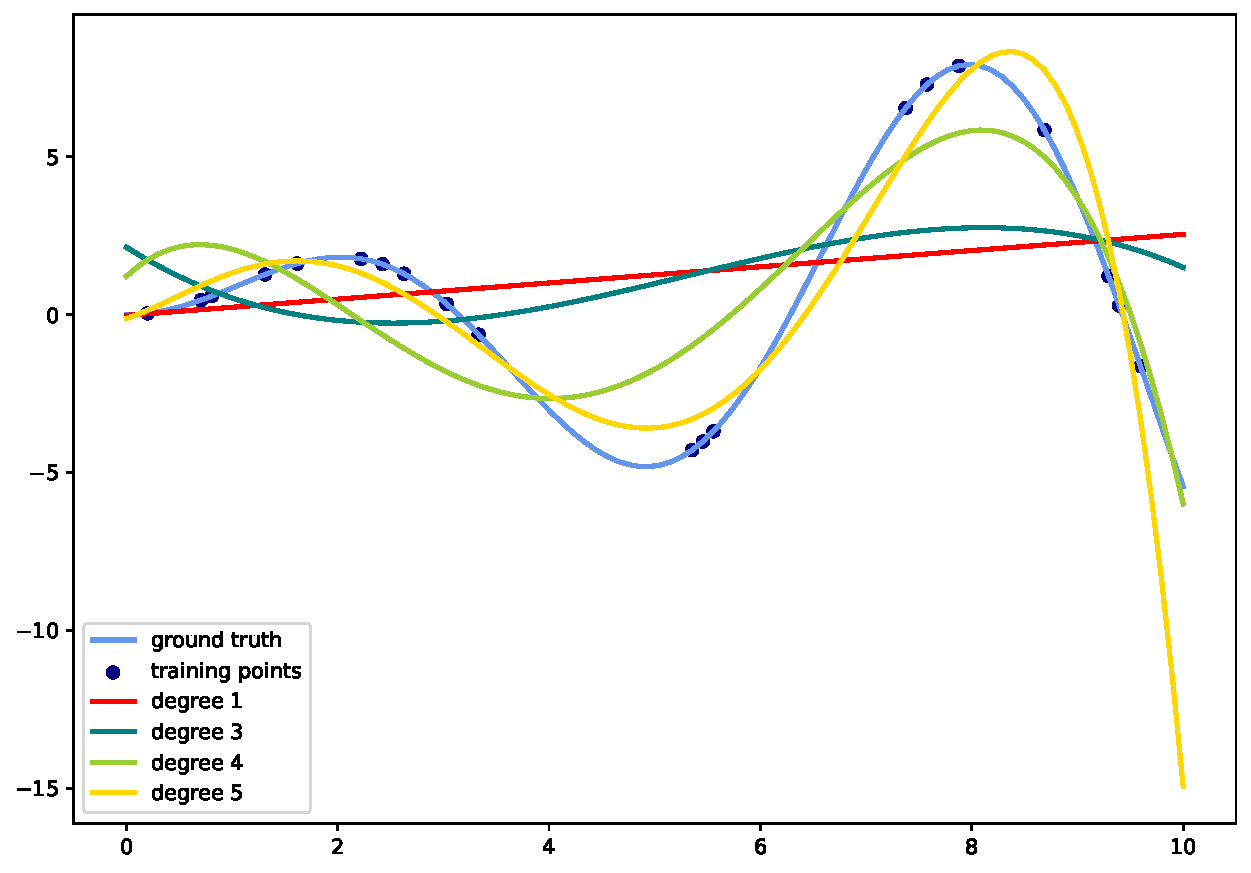
\includegraphics{Lecture0_accuracy_n_prediction_files/figure-beamer/cell-2-output-2.pdf}

Note that the number of parameters to be estimated increases + For
degree 1, \(f(x)=a_1x+a_0\) + For degree 2, \(f(x)= a_2x^2+a_1x+a_0\),
etc.
\end{frame}

\begin{frame}{Classification}
\phantomsection\label{classification}
When we have \emph{categorical responses} (e.g., ``high'',
``low'',``medium'') the our prediction problem become a
\textbf{classification problem}. Let's suppose that we are looking for a
estimate \(f\) basis of the \emph{training} observations
\(\{ (x_1,y_1), \ldots, (x_n,y_n)\}\) where \(y_i\) is a member of one
given class \(C_k\) (\(k\in \{1,\ldots,r\}\).

One common approach to quantify the quality of the estimate \(\hat{f}\)
is the \textbf{training error rate}, that is the proportion of
classification errors that we incurred during if we apply our estimate
\(\hat{f}\).

\begin{equation}
\frac{1}{n} \sum_{i=1}^n I_{y_i \ne \hat{y}_i}
\end{equation}

where \(\hat{y}_i\) is our prediction for the observation \(i\) by the
estimate \(\hat{f}\), and \(I_{y_i \ne \hat{y}_i}\) is the
\emph{indicator function} which is equal to 1 if the condition is true
(i.e.~\(y_i \ne \hat{y}_i\)) and zero elsewhere. Thus the expression on
the right is measuring the fraction of incorrect classifications.

As we did before, we can define the \textbf{test error rate} associated
with a set of previously unseen observations \((x_0,y_0)\) as

\begin{equation}
\mathrm{Average}(I_{y_0 \ne \hat{y}_0}) 
\label{eq:classtesterror}
\end{equation}

\begin{block}{Bayes classifier}
\phantomsection\label{bayes-classifier}
The test error rate given in (\ref{eq:classtesterror}) can be minimized
(on average) by a simple classifier that assigns \emph{each observation
the most likely class, given its predictor values}). So, for the test
observation with predictor vector \(x_0\) will belong to the class \(j\)
for which

\[
\mathrm{Pr}(Y=j | X=x_0)
\]

is largest. This classifier is refered to as \textbf{Bayes classifier}.

The Bayes classifier produces the lowest possible test error rate,
calles the \textbf{Bayes error rate}. In general the overall Bayes error
rate is given by

\[
1 - E \left( \max_{j} \mathrm{Pr}(Y=j|X) \right)
\]
\end{block}

\begin{block}{K-Nearest Neighbors}
\phantomsection\label{k-nearest-neighbors}
One of the problems with the Bayes classifier is that we normally don't
know the conditional distribution \(Y\) given \(X\). Thus, it becomes a
\emph{theoretical gold standard} which is unattainable.

\(K\)-nearest neighbors (KNN) in which given a positive integer \(K\)
and a test observation \(x_0\), the \emph{KNN} classifier first
identifies the \(K\) points in the trianing data that are the closests
to \(x_0\), represented by \(\cal{N}_0\). It then estimates the
conditional probability for class \(j\) as the fraction of points in
\(\cal{N}_0\) whose response values equal \(j\):

\[
\mathrm{Pr}(Y=j | X=x_0) = \frac{1}{K} \sum_{i \in {\cal N}_0} I_{y_i=j}
\]

Finally, KNN aplies Bayes rule and classifies the test observation to
\(x_0\) to the class with the largest probability.

\includegraphics{attachment:32d4a146-6c79-4f16-9c45-276be1ab69bb.png}\#\#\#\#
Example

Let's suppose we have two classes \(\circ\) of two colors and \(\times\)
represents the center of an unseen new point \(x_0\). And let's pick
\(K=3\). So the closests three points are inside or in the boundary of
the green circle. This circle has 2 blue and 1 orange point. Thus,
resulting in estimated probabilities of \(2/3\) for the blue and \(1/3\)
for the orange class.

Then, the \(\times\) point belongs to the blue class. When the same
procedure is applied to a sufficient number of points in the plane, we
get something like this

\includegraphics{attachment:f28d0390-b2a6-4db1-bed8-a32636827d8b.png}\#\#\#
Effect of \(K\)

The choice of \(K\) has a significant impact on the KNN classifier.

From this picture, we can see that when \(K=1\), the \emph{decision
boundary} is overly flexible (i.e.~almost classifies the dataset
``perfectly''). This case we expect that the classifier has low bias but
very high variance. On the other hand, when we have a high \(K\) (in the
picture \(K=100\)) we get almost linear classification, where low
variance and high bias is expected.

Just as we did with the other classifiers, we consider the variable
\(1/K\) as \emph{flexibility}

Thus, we observe the same \(U\) shape for the \emph{test error rate} and
decreasing \emph{training error rate} as the model tends to overfit
data. The dotted line represents the Bayes error rate.

For the case of \(K=10\) we have

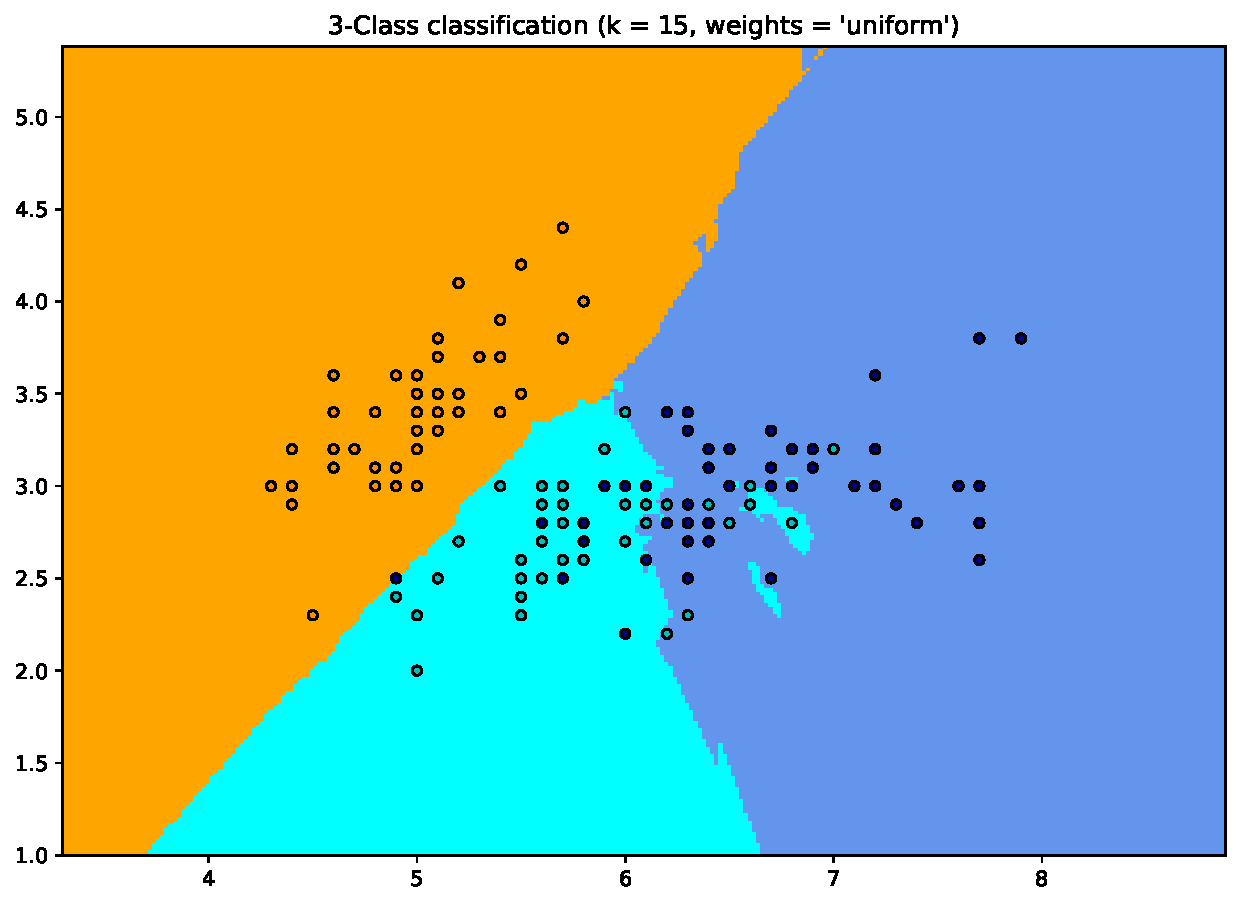
\includegraphics{Lecture0_accuracy_n_prediction_files/figure-beamer/cell-3-output-1.pdf}

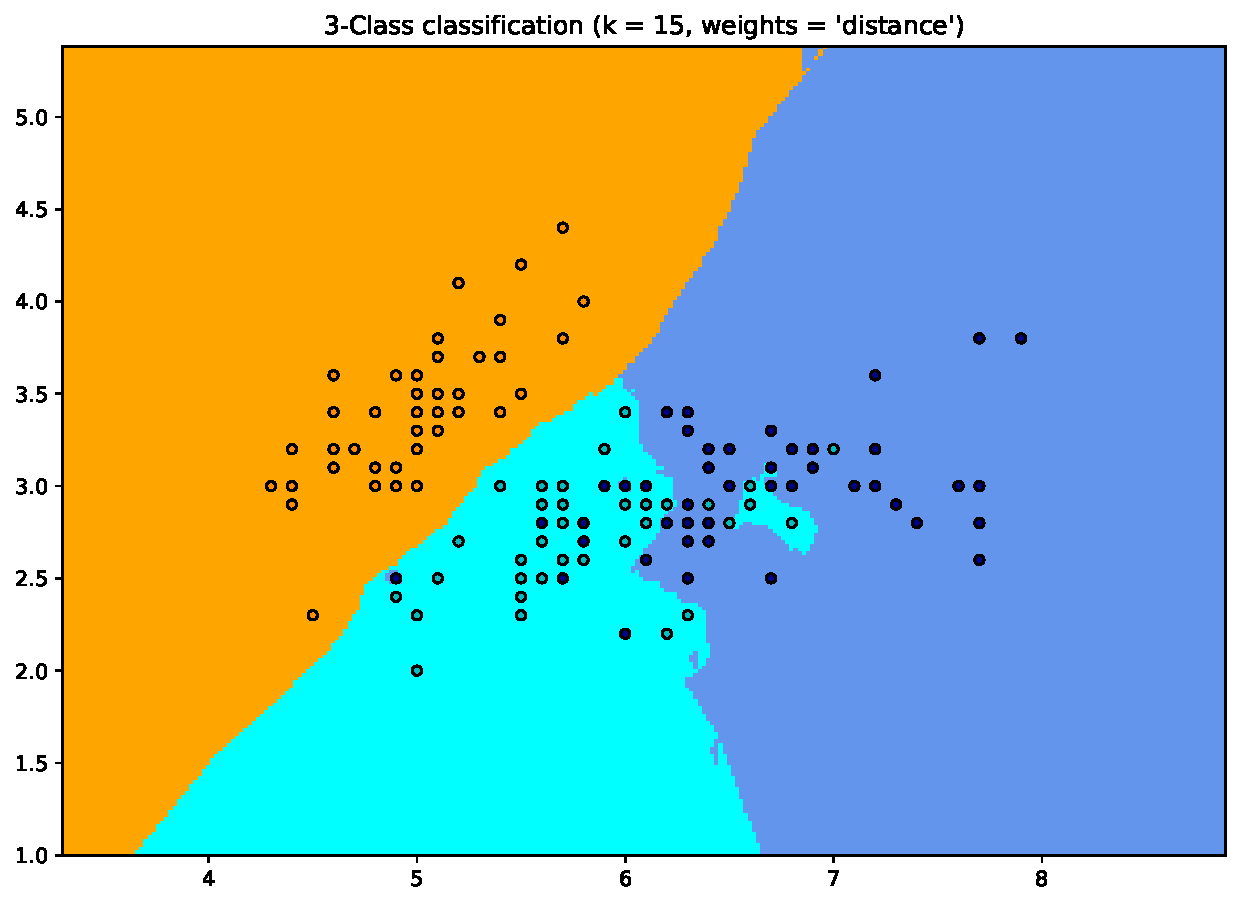
\includegraphics{Lecture0_accuracy_n_prediction_files/figure-beamer/cell-3-output-2.pdf}
\end{block}
\end{frame}




\end{document}
